\glsresetall    
\chapter{Introduction}
\label{ch:introduction}

% \glspl{llm} like GPT-4 \cite{openai_gpt-4_2024} and Flan-T5 \cite{chung_scaling_2022} sparked a revolution in the field of natural language processing tasks. These models are built on the transformer architecture \cite{vaswani_attention_nodate} and trained on extensive datasets scaled to billions of parameters, which leads to remarkable abilities in zero-shot learning, step-by-step reasoning, in-context learning, instruction following, human alignment, and tool manipulation \cite{yang_give_2024}. 

% Providing textual answers to user questions, relieve users of the cognitive effort of collecting the needed information from individual search results themselves.

% Question answering is a retrieval task more challenging than common search engine tasks because its purpose is to find an accurate and concise answer to a question rather than a relevant document. The difficulty is more acute in tasks such as story comprehension in which the target text is less likely to overlap with the text in the questions. For this reason, advanced natural language techniques rather than simple key term extraction are needed. \cite{Learning Question Classifiers by Xin Li}

% GraphRAG is still in its early stages \cite{peng_graph_2024}

% \section{Motivation}
% \label{sec:motivation}

% - Scholarly Literature Search is time-consuming and cognitively demanding, nowadays all research findings are communicated via digital scholarly articles, a practice often referred to as the document-centric approach \cite{jaradeh_open_2019-1,auer_towards_2018}
% - Research Knowledge Graphs can help to make research more efficient
% - But to query information from the graph is also demanding as the user is required to know the graph structure to traverse the graph to find related information 
% - Recent development in the literature unifies LLMs with Graphs to exploit the advantages from both: 
% -- LLM Advantages: General Knowledge, Language Processing, Generalizability
% -- Graph Advantages: Structural Knowledge, Accuracy, Deciseveness, Interpretability, Domain-specific Knowledge, Evolving Knowledge
% - Graph Retrieval Augmented Generation (GraphRAG) \cite{peng_graph_2024} has been established which utilizes LLMs to retrieve relevant knowledge from the graph given a natural language question
% - As shown by current approaches, adding a Graph to the Retrieval can improve the quality and reliability of answers generated by LLMs \cite{edge_local_2024, guo_lightrag_2024}
% - Most current graph retrieval approaches focus on general domains and it is unknown how they perform in the scholarly literature search task
% - However some research is starting on the scholarly domain \cite{jaradeh_question_2020,taffa_leveraging_2023,giglou_scholarly_2024}


% Need to add somewhere:
% - We developed a question taxonomy that with the goal: “The taxonomy is designed to classify the characteristics of questions posed to KGQA retrieval systems in the literature search domain, enabling the creation of diverse question sets that test a broad range of retrieval capabilities.”
% - We created HubLink, a new retrieval approach that leverages the structure of RKGs to improve the relevance and accuracy of retrieved contexts and be able to answer complex questions that are asked in the literature search.
% - We evaluated against baselines that are training free (as our approach) which means that they use pre-trained LLMs and do not require further fine-tuning or training of models. \cite{jiang_structgpt_2023}, \cite{sun_think--graph_2024}, \cite{wen_mindmap_2024}, \cite{sui_fidelis_2024}, \cite{baek_direct_2023}
% - Approaches like semantic parsing struggle because of: Semantic Parsing hat allerdings zwei bedeutende Herausforderungen wie von \textcite{gu_knowledge_2022} herausgestellt: \emph{Schema-Level Complexity} und \emph{Fact-Level Complexity}. Zunächst ist das Schema eines modernen \gls{kg} extrem reichhaltig was bedeutet, dass die Anzahl an Items eines Schemas mehrere tausend beinhalten kann. Beispielsweise hat der FREEBASE \gls{kg} über 8k an Schema items. 
% - Klar machen warum es sinnvoll ist das man Knowledge Graphen verwendet statt einfach direkt die Informationen zu embedden -> Auf Die Paper LightRag und MicrosoftGRAPH rag \cite{edge_local_2024, guo_lightrag_2024} verweisen die das zeigen. Also im Prinzip ist es in der Motivation schonmal wichtig klar zu machen warum der Ansatz gebraucht wird. Also das Sparql Generierung nicht aussreicht und das nur das Document Embedding auch nicht reicht

Today, almost all scholarly findings are communicated through digital scholarly articles, a practice often referred to as the document-centric approach \cite{jaradeh_open_2019-1,auer_towards_2018}. Although the transition from print to digital has significantly improved accessibility \cite{sompel_all_2009,bosman_scholarly_2017}, it still does not fully take advantage of modern digital technologies. In current research practice, each publication is treated as an isolated unit of knowledge, making it challenging to interlink related findings, methodologies, and underlying data. This isolation becomes especially problematic given the exponential growth of scientific literature \cite{bornmann_growth_2021}. Researchers must navigate an extensive body of text to identify relevant insights. This process is challenging due to the sheer volume of content and also the addition of inherent issues that plague text searches. For example, the lexical gap problem, in which misspellings, synonyms, abbreviations, ambiguous words, and the ignored word order hinder the effectiveness of searches \cite{li_unsupervised_2022}. Consequently, literature search becomes a time-consuming and cognitively taxing process, requiring careful crafting of search queries, manual sifting through countless documents, and painstaking synthesis of scattered evidence. 

Recently, \glspl{llm} have demonstrated powerful capabilities in understanding natural language, expressiveness, general knowledge, and generalization \cite{yang_give_2024}. In the context of \gls{qa}, integrating \glspl{llm} allows users to pose queries in natural language, with the system generating relevant answers. This is particularly interesting for scholarly literature search as it allows researchers to find answers to scientific resources by asking questions in natural language, effectively reducing manual effort. However, using the pre-trained internal knowledge of the \glspl{llm} is not sufficient because their answers may lack depth, be subject to hallucinations, and do not provide transparency regarding the underlying reasoning process \cite{yang_give_2024}. 

To mitigate these issues in the \gls{qa} setting, \gls{rag} has emerged, in which an external \gls{kb} is used to provide relevant context to the \gls{llm} to enhance the answer generation \cite{lewis_retrieval-augmented_2021}. In this framework, an indexing phase takes place where the collection of documents is split into text chunks, which are then converted into dense vector representations and stored in a vector store. At query time, the vector representation of the question is used to conduct a distance-based search in the vector space to find the most relevant text chunks. Although this approach can be applied to the scholarly literature search setting \cite{lu_dense_2024}, naive \gls{rag} encounters notable drawbacks. Retrieval can suffer from poor precision and recall, missing crucial context, or retrieving irrelevant information \cite{gao_retrieval-augmented_2024}. Furthermore, \glspl{llm} often struggle with noisy or misleading documents, fail to abstain from answering when relevant information is absent, perform poorly at integrating information across multiple sources, and are prone to accepting factual errors in the retrieved context \cite{chen_benchmarking_2023}.

An alternative to document-centric knowledge representation is to structure and interconnect representations of scholarly knowledge \cite{jaradeh_open_2019-1}. This can be achieved using \glspl{kg} where knowledge is curated from structured and unstructured sources \cite{verma_scholarly_2023}. Specifically for the academic domain, these graphs are referred to as \glspl{rkg} and offer a promising solution to structure and interlink scholarly information. With the aim of transforming scientific communication from document-centric to knowledge-centric \cite{auer_towards_2018}, \glspl{rkg} provide a structured and machine-readable representation of scholarly knowledge by taking into account the relationships between texts and the incorporation of structural information as additional knowledge \cite{peng_graph_2024}.

The unification of \glspl{llm} and \glspl{kg} is a relatively new research field that aims to utilize the advantages of both in various applications \cite{pan_unifying_2024}. One such application is \gls{kgqa}, where the integration of knowledge from a \gls{kg} to inform the \gls{llm} during inference is investigated \cite{banerjee_knowledge_2024,chakraborty_introduction_2021,chakraborty_introduction_2019,pan_unifying_2024,yani_better_2022,peng_graph_2024,jin_large_2024,feng_trends_2023,li_survey_2024,agrawal_can_2024,procko_graph_2024}. 
Although many \gls{kgqa} approaches have emerged, most of the approaches are focused on open-domain \gls{qa} and have not yet been tested in the scholarly field. Furthermore, approaches explicitly aimed at the scientific field focus primarily on \gls{sp} methods that automatically create structured queries from natural language queries using training examples \cite{banerjee_dblp-quad_2023, taffa_leveraging_2023, lehmann_large_2024, jiang_structure_2023, jaradeh_question_2020}. 

Despite being effective in controlled settings, \gls{sp} methods struggle to adapt to dynamically evolving \gls{kg} schemas, leading to poor performance when encountering previously unseen entities or relations. In addition, semantic parsing approaches face significant scalability challenges, including both schema-level and fact-level complexities \cite{gu_knowledge_2022}. These problems are exacerbated by the extensive schema richness of modern \glspl{kg}, which often encompasses thousands of schema items. Moreover, semantic parsing methods typically require manually curated training datasets, which are costly to produce and limit their applicability in real-world research environments, making the methods inconvenient to use. 

Consequently, we identify a research gap in applying alternative \gls{llm}-based strategies to the scholarly \gls{kgqa} task. Most alternative strategies are developed and evaluated on general-purpose graphs like Freebase or Wikidata \cite{peng_graph_2024}. However, these approaches cannot be easily adapted to the scholarly domain \cite{saikh_scienceqa_2022}. Moreover, current retrieval approaches often ignore the source diversity of retrieved information, potentially returning multiple pieces of information from the same publication, reducing the breadth of evidence needed for robust scholarly inquiries. Therefore, the scholarly domain remains underexplored within \gls{kgqa} research.

Motivated by these challenges, we argue that research on scholarly \gls{kgqa} should explore directions beyond semantic parsing to develop methods that do not require training or fine-tuning and can adapt to dynamically changing \gls{kg} schemas. Our thesis contributes a novel \gls{kgqa} retrieval approach that complies with the above-mentioned criteria. We rigorously evaluated the approach on a scholarly literature search task in a \gls{swa} setting against five state-of-the-art baseline \gls{kgqa} approaches on the \gls{orkg} to demonstrate its superiority in retrieval performance. We further contribute a new taxonomy for the classification of questions querying \gls{kgqa} systems for literature search. With these contributions, our aim is to advance research in the direction of \gls{kgqa} in the scholarly literature search domain.


% In summary, despite promising advances in \gls{grag} and \gls{kgqa}, the academic domain remains underexplored. Existing methods either depend on general purpose graphs that fail to capture the specific request of literature search or rely on semantic parsing methods that struggle with evolving and scaling \gls{kg} schemas. Therefore, more research is required to achieve a robust, scalable, and schema-agnostic retrieval approach tailored for scholarly \glspl{kgqa}.

% Although helpful, this document-centric approach still struggles with precision and recall in \gls{qa} tasks \cite{gao_retrieval-augmented_2024}.

% By encoding semantic and relational information, \glspl{rkg} facilitate sophisticated queries and structured retrieval that surpass traditional keyword-based methods. 

% Despite these advantages, effectively querying an \gls{rkg} remains challenging. Traditional methods such as manually crafting SPARQL queries require users to possess in-depth knowledge of the graph schema. Even with user-friendly interfaces like that of the \gls{orkg} \cite{jaradeh_open_2019}, navigating these graphs can be cumbersome, particularly for complex queries.


% into the \gls{rag} framework, forming what is now known as \gls{grag} \cite{peng_graph_2024, pan_unifying_2024}. \gls{grag} approaches leverage the structured, relational nature of \glspl{kg} to retrieve more relevant and interpretable contexts. A growing body of research demonstrates the effectiveness of these methods in various domains \cite{pan_unifying_2024,peng_graph_2024,jin_large_2024,feng_trends_2023,li_survey_2024,agrawal_can_2024,procko_graph_2024}.



% Furthermore, we observe that many current retrieval approaches require additional training or fine-tuning prior to the retrieval process. 
% This is a significant limitation, as it requires ground truth data, which is often unavailable. 
% We envision, that for useability in practice, a retrieval approach should be \enquote{plug-and-play}, meaning that it should not require any training or fine-tuning prior to the retrieval process. 
% As such, \emph{the approach should only require the \gls{rkg} and no additional ground truth data}. 


% Moreover, we identified that many current retrieval approaches are only considering the retrieval of single entities as oposed to complex natural language answers.

% Researchers are confronted with the task of navigating the immense growth of scientific literature \cite{bornmann_growth_2021}, which is made even more difficult as there is no dedicated database for scientific literature. As consequence, researchers have to use academic search engines to find relevant literature. 

% Traditional results from search engines include a list of links to information sources that may contain the answer to the question of the user. However, this approach requires cognitive effort from the user to collect the needed information from the individual search results. To relieve users of this effort, the design of result presentation from search engines has changed with the introduction of \glspl{llm} as illustrated in \autoref{fig:new_search_engine_results_page}. Instead of providing a list of links, the search engine now provides textual answers each linked to the source of the information \cite{gienapp_evaluating_2024}.

% \begin{figure}
%     \centering
%     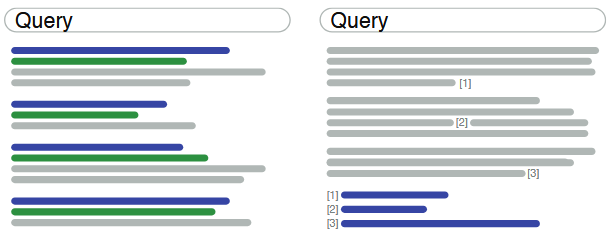
\includegraphics[width=1.0\linewidth]{figures/new_search_engine_results_page.png}
%     \caption{Change of results presentation in search engines \cite{gienapp_evaluating_2024}}
%     \label{fig:new_search_engine_results_page}
% \end{figure}

% The research community has proposed many QA systems, but to the best of our knowledge none focus on scholarly knowledge \cite{jaradeh_question_2020}

% TODO ADD Semantic Parsing Discussion:

% Semantic Parsing methods are early adopters for \gls{qa} on \glspl{kg}. These methods convert questions into a structural query such as SPARQL

% However, these methods heavily rely on the quality of generated queries. If the query is not executable, no answer will be generated. \cite{sui_fidelis_2024}
% Most important: Knowledge Base Question Answering: A Semantic Parsing Perspective
% Auch nochmal schauen warum Embeddingbasierte Ansätze Probleme hat
% Klar machen warum es sinnvoll ist das man Knowledge Graphen verwendet statt einfach direkt die Informationen zu embedden -> Die Paper LightRag und MicrosoftGRAPH rag verweisen die das zeigen. Also im Prinzip ist es in der Motivation schonmal wichtig klar zu machen warum der Ansatz gebraucht wird. Also das Sparql Generierung nicht aussreicht und das nur das Document Embedding auch nicht reicht

\section{Problem Statements}
\label{sec:problem_statements}

\gls{kgqa} approaches show promising results in the \gls{qa} setting. However, most approaches are applied to the general-purpose domain and are not tailored to scholarly content. Those approaches that target scholarly \gls{kgqa} often rely on \gls{sp} techniques that struggle with dynamically evolving schemas and often require training data. As a result, the potential of applying \gls{kgqa} to support effective scholarly search remains largely untapped, leading to our first problem statement:

\begin{enumerate}[label=\textbf{P\arabic*}, leftmargin=2.5em]
    \item \label{enum:p1} There is an underexplored potential in applying \gls{kgqa} in the scholarly domain to help researchers find relevant literature faster and more reliably. Initial approaches show promising results, but they struggle with evolving schemas and often require training data. This problem hinders the practical application of \gls{qa} systems on the scholarly literature search task in real-world scenarios. 
\end{enumerate}

The application of a \gls{kgqa} approach to an \gls{rkg} has the potential to help researchers in finding related literature faster and more reliably. This is made possible through the natural language capabilities of \glspl{llm} that allow researchers to ask for information of interest using natural language rather than having to manually search for it. 

To assess whether such a \gls{kgqa} system is capable of answering desirable questions for literature search, a taxonomy can help. Such a taxonomy classifies questions according to their complexity and the retrieval capabilities required to arrive at the answer. Although there are existing taxonomies, such as in DBLP-QuAD \cite{banerjee_dblp-quad_2023} and SciQA \cite{dubey_lc-quad_2019} for \gls{kgqa} or the works provided by \textcite{li_learning_2002} and \textcite{singhal_att_1999} for general \gls{qa}, they often propose divergent classification schemes. Without a synthesized and domain-relevant taxonomy, it is challenging to assess whether a given system can handle the full range of question types and retrieval complexities found in scholarly search tasks. Such a taxonomy can be helpful to guide the development of robust \gls{kgqa} datasets used for benchmarking and tailored to the needs of researchers, leading to our second problem statement:

\begin{enumerate}[label=\textbf{P\arabic*}, leftmargin=2.5em, start=2]
    \item \label{enum:p2} There is a lack of a taxonomy that allows the classification of the characteristics of questions posed to \gls{kgqa} retrieval systems in the scholarly literature search task. This hinders the creation of diverse question datasets to test the retrieval capabilities of \gls{kgqa} approaches on different \gls{rkg}. 
\end{enumerate}

Using such a taxonomy and applying it to the scholarly literature search task can help in the process of creating \gls{qa} datasets to reliably determine whether a retrieval approach is able to meet its challenges.

% The primary objective of this thesis is to design, implement, and evaluate a new training-free and schema-agnostic retrieval approach that takes advantage of the inherent structure of \glspl{rkg} to improve the quality and reliability of \gls{qa} systems for literature search tasks.

% Although HubLink is designed to be domain-agnostic, this work focuses on its application within the scholarly domain, using the \gls{orkg} as a representative \gls{rkg} for empirical evaluation.

% HubLink is built on the insight that \glspl{rkg} organize knowledge around publication nodes, forming natural \enquote{hubs} of semantically related information. By exploiting this structure and incorporating source diversity during retrieval, HubLink addresses key challenges in scholarly question answering particularly those involving multiple constraints and the need to aggregate evidence from various sources.


\section{Objective and Research Questions}

After discussing the potential benefits and importance of utilizing \gls{kgqa} to enhance the search of scholarly literature and addressing the issues with existing approaches (\textbf{P1}) together with the evaluation of \gls{kgqa} retrieval systems (\textbf{P2}), we establish the research objective of this thesis as follows:

\begin{tcolorbox}
    \textbf{Research Goal:} Design a training-free and schema-agnostic retrieval approach leveraging \glspl{rkg} and pre-trained \glspl{llm} that enhances the quality, transparency, and reliability of context retrieval in \gls{kgqa} systems specifically tailored to scholarly literature search tasks. Additionally, construct a taxonomy for classifying questions posed to \gls{kgqa} retrieval systems to support the assessment of capabilities and performance of such systems in the scholarly literature task.
\end{tcolorbox}

A new retrieval approach that does not rely on a \gls{kg} schema and is training-free would benefit the exploration of the potential that such systems can have in literature search tasks. This addresses the first problem, \textbf{P1}. Furthermore, a taxonomy for characterizing questions in \gls{kgqa} retrieval can help to guide the construction of \gls{kgqa} datasets used for benchmarking retrieval systems. This addresses the second problem, \textbf{P2}.

To achieve this goal, the thesis is guided by research questions. The first question concerns the design and technical foundation of the new \gls{kgqa} retrieval approach:

\begin{enumerate}[label=\textbf{RQ\arabic*}, leftmargin=2.5em]
    \label{enum:rq1}
    \item How can a schema-agnostic retrieval algorithm leveraging an \gls{rkg} and a pre-trained \gls{llm} be developed for the \gls{kgqa} setting to effectively integrate diverse scholarly sources, adapt to evolving schemas and account for the provenance of information during retrieval without relying on training data?
\end{enumerate}

This research question addresses the first problem (\hyperref[sec:problem_statements]{\textbf{P1}}) as it directly targets the limitations of current scholarly \gls{kgqa} approaches. By developing a schema-agnostic and training-free approach, it explores the potential of retrieval without relying on the schema of the \gls{rkg} and thus is scalable and dynamically adaptable. Furthermore, without the requirement of a training dataset, the approach becomes more conveniently applicable and thus more relevant to apply in a real-world use case. Moreover, accounting for the provenance of information during inference is a critical aspect of scholarly literature search, as it supports the generation of complete, transparent, and balanced results. Provenance awareness helps prevent over-reliance on a single source and encourages the integration of diverse perspectives, ensuring that results capture complementary aspects that may not be covered by only one source alone.

The second question is related to understanding the nature of questions targeting scholarly \gls{kgqa} systems. Since the search for scholarly literature covers a wide range of information needs, it is important to characterize these needs and ensure that the evaluation datasets reflect their diversity, which can be achieved using a taxonomy. This motivates the following question:

\begin{enumerate}[label=\textbf{RQ\arabic*}, leftmargin=2.5em, start=2]
    \label{enum:rq2}
    \item How can existing general \gls{qa} and \gls{kgqa} taxonomies be synthesized and extended to form a comprehensive taxonomy tailored to define the characteristics of questions posed to \gls{kgqa} retrieval systems for the literature search task?
\end{enumerate}

The second research question addresses the second problem (\hyperref[sec:problem_statements]{\textbf{P2}}). A taxonomy of this kind offers insight into the extent of capabilities that a \gls{kgqa} approach has in answering questions posed with regard to the scholarly literature search task. In our thesis, we apply this taxonomy to create \gls{kgqa} datasets that allow the evaluation of our proposed \gls{kgqa} approach and understand its capabilities.


% Generalisierbarer Prozess zur Taxonomie erstellung (Operationalisierungsschritte bei Usman Fehlen), die Skripte zur Erstellung
% Welche Anforderungen, die Instanzierung auch selbst?, 

% In this master thesis, we develop a novel retrieval approach for the scholarly \gls{kgqa} task. To support the evaluation of this method, we further provide a question taxonomy for \gls{kgqa} retrieval systems and semi-automatically created \gls{qa} datasets. To that end, we propose to take advantage of the unique structural properties of an \gls{rkg} to conduct a source aware retrieval. In this context, the contributions provided by the master thesis are as follows:

% In this master thesis, we investigate the potential of using a \gls{kgqa} approach to support scholarly literature search using a schema-agnostic and training-free approach.

\section{Research Contributions}

This thesis provides the following contributions to investigate the potential of using \gls{kgqa} to support scholarly literature search:

\begin{enumerate}[label=\textbf{C\arabic*}, leftmargin=2.5em]
    \item \label{enum:c1} A novel \gls{kgqa} retrieval approach named \emph{HubLink}, which is a schema-agnostic and training-free method designed to conduct source-aware inference on \glspl{kg}.
    \begin{enumerate}[label=\textbf{C1.\arabic*}]
        \item \label{enum:c1.1} The \gls{sqa}-framework, which enables modular testing of \gls{rag} pipelines with various \glspl{kg} and retrieval approaches and the semi-automatic generation of \gls{kgqa} datasets.
        \item \label{enum:c1.2} Implementations of five training-free and schema-agnostic \gls{kgqa} retrieval approaches from the existing literature adapted for use on the \gls{orkg}.
        % \item \label{enum:c1.3} Experimental evaluations against state-of-the-art, non-semantic parsing, and training-free baselines, demonstrating the superior performance of HubLink, particularly on complex questions.
    \end{enumerate}
    \item \label{enum:c2} A question taxonomy for classifying questions targeting scholarly \gls{kgqa}, facilitating the development of diverse \gls{kgqa} datasets to evaluate the performance and capabilities of retrieval systems.
    \begin{enumerate}[label=\textbf{C2.\arabic*}]
        \item \label{enum:c2.2} A systematic question taxonomy construction process to synthesize existing knowledge from the literature, emphasizing replicability, transparency, and validation.
    \end{enumerate}
    \item \label{enum:c3} A new \gls{kgqa} dataset for the \gls{orkg} featuring four variants for different graph schemas, designed to benchmark the performance and robustness of \gls{kgqa} systems across a wide range of question types in the scholarly literature search task.
\end{enumerate}

The primary contribution of this thesis is HubLink (\textbf{C1}), a novel \gls{kgqa} approach that conceptually decomposes the graph into structures termed \emph{hubs}. Each hub is individually evaluated to determine its relevance in answering the provided question, with a subsequent generation of partial answers for each relevant hub. These partial answers are then synthesized into a final answer. This modular approach enables the retrieval process to be source-aware, schema-agnostic, and training-free. To support this contribution, a framework (\textbf{C1.1}) that implements a modular and configurable \gls{rag} pipeline to benchmark \gls{kgqa} approaches on different \glspl{kg} is contributed. Subsequently, implementations of five established state-of-the-art \gls{kgqa} approaches from the literature are provided, which were previously tested only in open-domain settings. Their implementations were adapted (\textbf{C1.2}) for compatibility with the \gls{orkg} and tested with regard to their performance against our novel HubLink approach in an extensive evaluation.

Furthermore, a question taxonomy (\textbf{C2}) is contributed, which enables the classification of questions specifically targeting \gls{kgqa} for the scholarly literature search task. This facilitates the creation of diverse and complex \gls{kgqa} datasets incorporating questions designed to test various capabilities of \gls{kgqa} approaches. To support this contribution, a taxonomy construction process (\textbf{C2.1}) is provided that systematically synthesizes knowledge from the literature and operationalizes the generation of taxonomies, complete with tool support for easy application.

Finally, new \gls{kgqa} datasets (\textbf{C3}) for the \gls{orkg} are contributed, which are based on an \gls{swa} schema and the question taxonomy (\textbf{C2}). Consequently, the datasets include a variety of questions that target different retrieval capabilities to thoroughly test \gls{kgqa} approaches. In addition, the datasets are based on six distinct use cases for the scholarly literature search task to ensure relevance to real-world scenarios and relate to four different graph variants corresponding to different graph schemas, to evaluate the schema-agnostic property and robustness of \gls{kgqa} approaches.



% The first contribution (\textbf{C1}) is a taxonomy specifically designed to classify the characteristics of questions posed to \gls{kgqa} retrieval systems in the scholarly literature search domain, enabling the creation of diverse question datasets that test a broad range of retrieval capabilities.


% To address this gap, we propose HubLink, a novel retrieval approach that takes advantage of the unique structural properties of \glspl{rkg}. In \glspl{rkg}, information about publications is naturally grouped into subgraphs. HubLink exploits this observation by pre-embedding each subgraph into so-called hub structures using a pre-trained embedding model during an offline indexing step. In this step, each subgraph is decomposed into distinct content levels that preserve both semantic and structural context. 

% At query time, the input question is similarly decomposed and encoded. HubLink retrieves the most relevant hubs through embedding similarity, assembles partial answers from each, and consolidates them into a final response. Crucially, HubLink also tracks the source of each retrieved piece of information, allowing the system to draw on multiple publications to provide diverse evidence. This is particularly important for complex scholarly questions that involve multiple constraints and require the synthesis of methodological details or results from different sources. We hypothesize that leveraging \gls{rkg} structure while maintaining source diversity fosters more accurate and transparent answers.

% To support robust evaluation, we also contribute a question taxonomy specifically designed to characterize the types of question posed to \gls{kgqa} retrieval systems in the literature search domain. This taxonomy enables the creation of diverse question datasets that test a broad range of retrieval capabilities. Using this framework, we semi-automatically generated new scholarly \gls{qa} datasets for the \gls{orkg} that reflect real-world literature search scenarios based on common use cases, ensuring that our evaluation covers realistic, relevant and diverse scholarly information needs.

% Our experiments, conducted on the \gls{orkg}, show that HubLink outperforms state-of-the-art non-semantic parsing and training-free baselines including StructGPT \cite{jiang_structgpt_2023}, Think-on-Graph \cite{sun_think--graph_2024}, MindMap \cite{wen_mindmap_2024}, Fidelis \cite{sui_fidelis_2024}, and DiFaR \cite{baek_direct_2023}, especially on complex questions involving multiple constraints and relational paths.

% In summary, we demonstrate that a retrieval approach such as HubLink can advance scholarly literature search by integrating the structured advantages of \glspl{rkg} with the natural language understanding capabilities of \glspl{llm}. This minimizes the time to locate relevant information, lessens the cognitive load for researchers, and facilitates accessibility. Therefore, this work contributes to the development of more effective workflows in academic research.

% In doing so, we take a step toward knowledge-based scientific communication, where the semantic organization of research data, combined with powerful language models, enables more efficient exploration of the rapidly expanding scholarly landscape. By reducing the burden of manual literature searches, our aim is to contribute to more productive, transparent, and wide-reaching scientific research.

\section{Thesis Outline}

After the introduction, the remainder of the master thesis is structured as follows: 

\textbf{\autoref{ch:fundamentals}} establishes the fundamental concepts upon which the research is built. This chapter introduces \glspl{kg}, with a specific focus on \glspl{rkg}. It further explains the \gls{orkg}, which is the graph used to conduct our experiments on. The chapter then continues with an explanation of \gls{kgqa}, the primary research field toward which this work is contributing. Furthermore, it includes an explanation of \glspl{llm}, covers \gls{grag}, \gls{ann} search, and a range of evaluation metrics relevant to retrieval and generation components. Finally, the chapter explains the concept of taxonomies, including their formal definition, development approaches, and evaluation methods.

\textbf{\autoref{ch:related_work}} provides a comprehensive review of existing literature relevant to this thesis. It first examines \gls{kgqa} approaches that utilize \glspl{llm} in the scholarly and open domains. The discussion then continues with taxonomy development and question classification, covering systematic approaches to taxonomy construction and evaluation, alongside question classification for scholarly \gls{qa} on \glspl{kg}. Finally, it examines the benchmarking of \gls{kgqa} systems, including datasets targeting open-domain and scholarly domain \glspl{kg}, and methodologies for \gls{qa} dataset construction.

\textbf{\autoref{ch:hublink}} presents our primary contribution of this thesis: \emph{HubLink}. It provides an overview of the HubLink approach, detailing the indexing, retrieval, and generation phases. It then proceeds to explain the formal definitions of key concepts of the approach, before explaining the approach in detail using pseudocode. In addition, the chapter outlines the challenges and design rationale for decisions made during the development of the approach. Finally, the chapter concludes with a discussion on the generalizability, scalability, index updating mechanisms, and limitations.

\textbf{\autoref{ch:taxonomy_construction_approach}} outlines the systematic process proposed in this thesis for the creation of taxonomies by synthesizing knowledge from the literature. The chapter begins with an evaluation plan that utilizes an \gls{gqm} model to facilitate the evaluation of a taxonomy. Subsequently, the iterative development process is outlined, which encompasses planning, literature survey, extraction of relevant concepts, clustering of these concepts, relevance assessment, the actual taxonomy construction and refinement stages, validation of the taxonomy, and finally, its application. The chapter also describes construction artifacts and discusses the limitations inherent in the proposed methodology.

\textbf{\autoref{ch:question_catalog}} details the application of the proposed systematic taxonomy construction approach, by creating a \gls{kgqa} retrieval taxonomy, aimed at the classification of questions for scholarly literature search. The chapter starts with the planning and a systematic literature survey, before describing the extraction of classes, including their distribution by category, domain, publication year, and citation metrics. Then, the clustering of extracted classes, including deduplication and categorization processes, is explained, followed by a relevance assessment of these clusters. Following this, the iterative construction and refinement of the taxonomy through three increments are presented. The chapter then systematically describes the categories and classes of the final taxonomy, before its application on \gls{swa} research questions is demonstrated. 

\textbf{\autoref{ch:implementation}} introduces the \gls{sqa} framework, central for the implementation of the \gls{kgqa} approaches, the creation of the \gls{kgqa} datasets, and the execution of the experiments. Furthermore, the chapter details the implementation of HubLink and the baselines \gls{kgqa} approaches, also describing the selection process by which the approaches have been chosen. The chapter further specifies the methods for accessing and populating the \gls{orkg}.

\textbf{\autoref{ch:experimentation_preliminaries}} sets the stage for the experimental evaluation of the HubLink approach against the baseline approaches. The chapter outlines the overall evaluation concept and describes the software and hardware environment used for the experiments. Furthermore, the creation of the \gls{kgqa} datasets, detailing the use cases for scholarly literature search, an overview of content granularity, and the dataset creation process is described. Following this, the evaluation framework and metrics are specified, including the evaluation targets and a detailed evaluation plan using the \gls{gqm} model. 

\textbf{\autoref{ch:parameter_selection_process}} details the methodology and results of the parameter selection process, which has been applied to select the configurations for the HubLink approach and the selected baseline methods. The chapter begins with the planning of the process, before presenting the results for the approaches HubLink, DiFaR, FiDeLiS, and Mindmap, each including their base configuration, parameter ranges explored, and the final selected parameters.

\textbf{\autoref{ch:experimentation}} presents and discusses the results of the comprehensive evaluation of the HubLink approach against the baseline methods. The evaluation is divided into two main parts: evaluating retrieval quality and evaluating answer alignment. The retrieval quality assessment examines the improvement of retrieval accuracy and relevance, the impact of operation complexity, applicability to different scholarly literature search use cases, the impact of type information in the question, robustness to structural and lexical variability in the graph schema, analysis of runtime and \gls{llm} token consumption, and the environmental sustainability impact. The answer alignment evaluation focuses on the semantical and factual consistency of generated answers, the generation of relevant answers, adherence to instructions provided in the question, and the consistency of generated answers with the retrieved context. The chapter concludes with a detailed discussion of the evaluation results.

\textbf{\autoref{ch:conclusion}} summarizes the key findings of the thesis and reflects on the research objectives and questions. It revisits the research questions posed at the beginning of the thesis, providing answers based on the research conducted and contributions made and concludes by discussing avenues for future work.